\chapter{Video codecs}

Codecs are algorithms used to compress video/image/sound data to reduce the
bandwidth required in streaming, or to reduce storage space required to archive
them. The higher the compression ratio, the more computational demand is
required. There are different standards, Fig.\ref{fig:codec_standards}.

\begin{figure}[hbt]
  \centerline{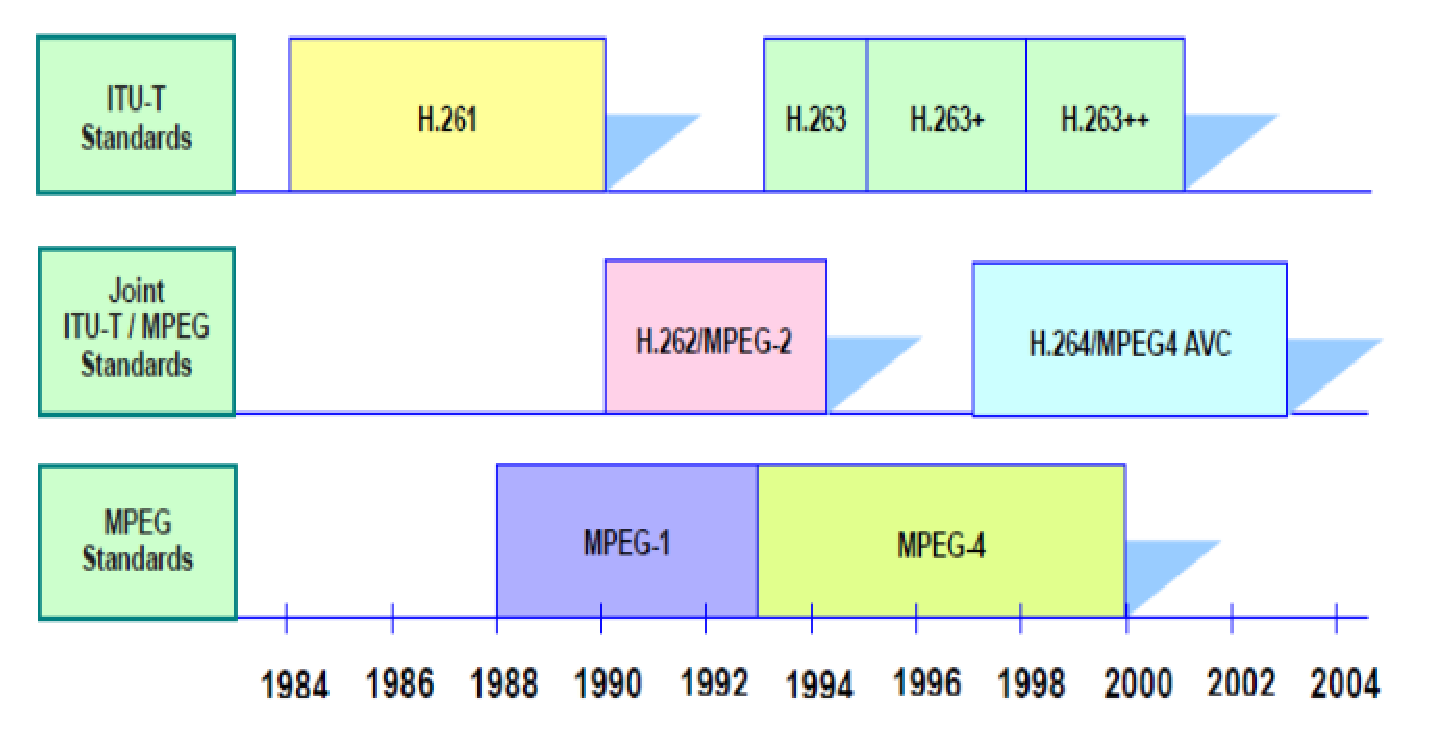
\includegraphics[height=5cm,
    angle=0]{./images/codec_standards.eps}}
\caption{Progression of ITU-T (International Telecom Union) and MPEG (Moving
Picture Experts Group) standards}
\label{fig:codec_standards}
\end{figure}

Pictures are encoded in either
\begin{enumerate}
  \item Y'CbCr: Y (luminance), and two color difference components (CB and CR).
  Y, CB, CR components are each function of the standard chrominance components
  (red, green, blue)
\end{enumerate}
You're recommended to read Sect.\ref{sec:H.261} first.


\section{Algorithms}

They use either vector quantization, or discrete cosine transform (DCT)

\subsection{Vector quantization}

Use in: Cinepak codec (Sect.\ref{sec:Cinepak})

\subsection{Wavelet-based codec: Discrete cosine transform (DCT)}

DCT is the basic for many algorithms in video/audio signal coding. DCT is
a Fourier-related transform, like discrete Fourier transform (DFT), but only for
real numbers.

Why {\bf cosine} is more efficient than sine function?




\section{Color-spaces}

Colors are mathematically represented in computers using a color model. A color
model is a tuple of numbers, typically in a group of 3 or 4 components. The
value of each component represents a color value. However, the exact color for
each value is ambiguous. This requires an {\bf absolute color space}. This makes
sure, using the same color tubple, it gives the exact output on every device
(monitor, printer). 

Any color can be represented as a mixture of a few primary colors, e.g: RGB
(Red,Green,Blue) or CMYK (Cyan, Magenta, Yellow, Black) or HSV (Hue,
Saturation, brightness Value). The collection of all colors can be represented
is a color-space. 

Depending on the size of each component (8-bit or 16-bit), the number of colors
can be represented (or the size of the color-space) are different.

To calculate the color, from the component values, there are different ways



Rec. 601, Rec. 709, SMPTE-170, SMPTE-240, and sRGB.


\url{http://en.wikipedia.org/wiki/Color_space}


\section{Chroma subsampling}
\label{sec:chroma_sampling}


\url{http://en.wikipedia.org/wiki/Chroma_subsampling}

\section{On2 company: TruMotion to VP}
\label{sec:TruMotion_VP}

On2 was acquired by GOOGLE in Feb, 2010. On2 focus on developing video codec
technology.
\begin{itemize}
  \item TrueMotion S: full motion video sequences (initialy with
  hardware-implementation of the codec only, and then software version:
  TrueMotion-S Compressor).
  
  Other software-based codec competitors: Cinepak and Intel Indeo.
    
  \item TrueMotion RT: real-time (RT) capture and process digital video
  \item VP3.2: was released to open-source community in 2001. Theora is a folk
  of this codebase VP3.2 (Sect.\ref{sec:Theora}). This is comparable to MPEG-4
  Part 2 (Sect.\ref{sec:MPEG4-Part2})
  
  \item VP4/VP5:
  
  \item VP6: introduced in 2003, and the implementation of this are
  \verb!Libvp62! (later stopped) and \verb!libavcodec!.  
  
  IMPORTANT: libavcodec57 and \verb!libavcodec-extra57! are conflicting each other, we only keep one, e.g. 
  \verb!libavcodec-extra57!.
  
  \item TrueMotion VP8 (published in 2008): after acquired by Google, it was
  made open-source in 2010 (BSD license).
  
  \item VP9: is open, loyalty free video compression standard developed by
  Google. It reduces bit-rate by 50\% compared to VP8 while keeping the same
  video quality. It uses superblocks of 64x64 pixels, with quadtree coding
  structure. It supports different colorspaces: Rec. 601, Rec. 709, SMPTE-170,
  SMPTE-240, and sRGB. VP9 has 2 profiles: {\bf profile 0 } (4:2:0 chroma
  subsampling) and {\bf profile 1} (addition support to 4:2:2 chroma
  subsampling, alpha-channel, depth-channel).
  
  Google Chrome v25 now support the decoder for VP9; ;and Chrome
  v29.0.1547 has full support for VP9. Firefox v28 supports VP9.
\end{itemize}

\section{Ogg Theora (open-source)}
\label{sec:Theora}

Theora is a free lossy video compression format developed by Xiph.org
Foundation, derived from VP3.2 codec (Sect.\ref{sec:TruMotion_VP}). 

Library: \verb!libtheora! is a reference implementation of this codec.


Theora vs. H.264:
\url{http://arstechnica.com/information-technology/2010/02/ogg-theora-vs-h264-head-to-head-comparisons/}

\section{Cinepak}
\label{sec:Cinepak}

Cinepak is lossy video codec, that encode video 320x240 at 1x (150KB/s) in
CD-ROM. This allows the video to be playable on slow CPUs, e.g. 12.5 MHz 68000.

Vectors are 2x2 pixel block which can be either 4 luminance values (grayscale),
or 4 luminance and 2 chrominance values (4:2:0 chroma subsampling).

File size is 70\% larger than those of the same quality MPEG-4 Part 2 or Theore
files.

\section{Indeo}

Indeo was developed by Intel in 1992, sold to Ligos in 2000. It's one of the
first codecs with full-video playback without using hardware accelerator. It
uses Y'CbCr 4:2:0 colorspace. Indeo codec is {\it assymmetrical}, as encoding
takes more time than decoding.

It is surpassed by MPEG codecs and others. The Windows implementation of the
codecs contain several security that may harm your computer if the files have
virus. Nowdays, in Windows 7, to enable the
playback of files in Indeo format, we can type
\begin{verbatim}
regsvr32 ir50_32.dll
\end{verbatim}

Indeo Video Interactive (IVI) is the wavelet-based codec
\url{https://www.siggraph.org/education/materials/HyperGraph/video/codecs/IVI.html}.
It only support 16-bit depths

\section{MPEG4}

\subsection{MPEG-4 Part 2}
\label{sec:MPEG4-Part2}

MPEG-4 Part 2 is known as MPEG-4 Visual, as it is a video compression format.

\begin{framed}
\textcolor{blue}{The term MPEG-4 refers to the collection of methods defining
compression standard for both visual and audio digital data} (ISO/IEC 14496,
introduced in 1998). MPEG-4 is still an evolving standard, and is divided into
multiple parts. MPEG-4 just defines the specs or the standards, and it's upto
developers to implement which features they want. So, they define the concept of
``profiles'' and ``levels'', so that a group of features are collectively
defined and the developers need to implement features in groups.

\end{framed}


\section{H.261}
\label{sec:H.261}

H.261 is the first standard from the H.26x family \citep{vetrivel2010}. It's
also the first truly digital video coding standard. H.261
was the standard defined to transmit video (i.e. encoding + decoding) by ITU
over PSTN (Public Switched Telephone Network) on which the data rates are
multiple of 64Kbps, i.e. $p\times 64$ kbits/sec. The value of $p$ in the range 1
to 30. 

The basic processing unit is called a {\bf macroblock}. Data for each macroblock
consists of a macroblock header followed by data for blocks. Data are organized
into blocks, then grouped into macroblocks, Fig.\ref{fig:YCbCr_H261}. Each
macroblock consists of a 16x16 array of {\it luma samples} and two 8x8 arrays of
{\it chroma samples}, using 4:2:0 sampling and YCbCr color-space.

\begin{figure}[hbt]
  \centerline{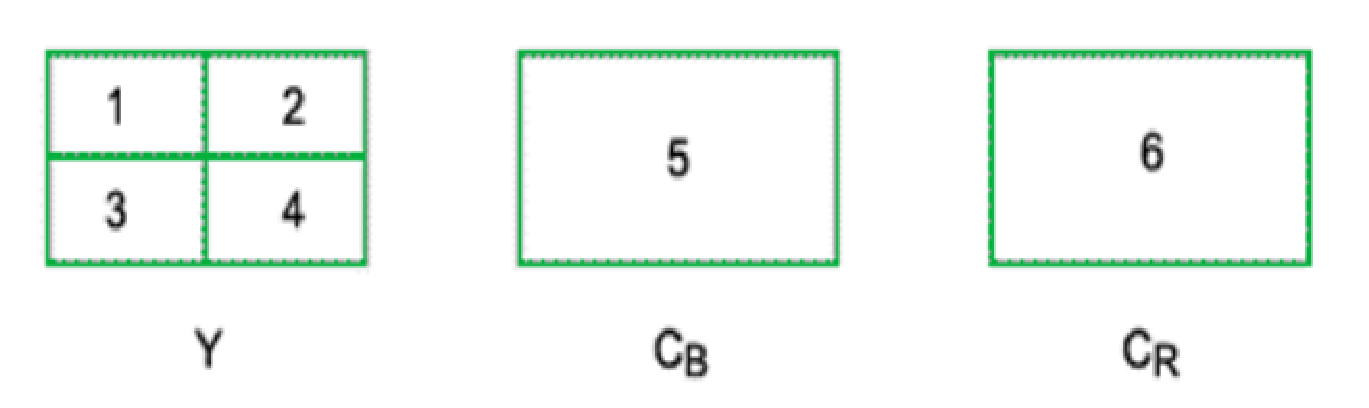
\includegraphics[height=5cm,
    angle=0]{./images/YCbCr_H261.eps}}
\caption{Data block within a macroblocks under H.261}
\label{fig:YCbCr_H261}
\end{figure}

H.261 supports 2 picture formats only (i.e. two video frame sizes): CIF (Common
Intermediate Format) has 288 lines by 360 pixels/line of luminance information
and 144 x 180 of chrominance information; and QCIF (Quarter Common Intermediate
Format) which is 144 lines by 180 pixels/line of luminance and 72 x 90 of
chrominance. Both used 4:2:0 sampling scheme (Sect.\ref{sec:chroma_sampling}).


As H.261 is optimized only for low data rates, H.261 doesn't work well over
Frame Relay or TCP/IP Internet. So, H.262 was developed.

\section{H.263}

H.263 was developed to work well for a wide range of bit rates, i.e. not limited
to 64Kbps like H.261. H.263 supports 5 picture formats: CIF, QCIF, SQCIF, 4CIF,
and 16CIF. 

Sorensen Spark is an implementation of the H.263 codecs, to use in Flash video
and Adobe Flash files. Flash Player 6 and 7 use Sorensen Spark; while Flash
Player 8 switch to VP6 (Sect.\ref{sec:TruMotion_VP}).


\section{H.264 (or H.264 AVC or MPEG-4 Part 10)}
\label{sec:H.264_AVC}

H.264 (MPEG-4 Part 10) is the world most popular video codec (Blu-ray discs, TV
broadcasting (satellite and cable)). It was jointly developed by International
Telecommunications Union (as H.264) and International Organization for
Standardization/International Electrotechnical Commission Moving Picture Experts
Group (as MPEG-4 Part 10, Advanced Video Coding, or AVC). H.264 or H.264 AVC is
used interchangable. H.264 was incorporated in Flash in 2007 (Apple), and
Silverlight in 2008 (Microsoft). 

As using H.264 needs to pay license fees to MPEG-LA, not many webbrowser and
video-providing website choose to support this codec
\url{http://shaver.off.net/diary/2010/01/23/html5-video-and-codecs/}. In
webbrowsers, H.264 playback is supported in Safari browser and Microsoft IE9 via HTML5 tag, and Google Chrome 11.0.696.16
beta.

H.264 video is encoded with audio compressed with AAC (Advanced Audio Coding)
codec, which is an ISO/IEC standard (MPEG4 Part 3).

H.264 is a specs, and thus can have different implementation, with different
levels of quality and configurability. Examples of them are
\begin{enumerate}
  \item x264 codec: free
  \item Apple codec: used in Apple Compressor and QuickTime Pro
  \item MainConcept codec: licensed by Adobe, Microsoft, Rhozet, Sorenson Media
  and Telestream 
\end{enumerate}

When using H.264 codecs, there are two main things you need to select: Profiles
and Levels
\begin{itemize}
  \item A profile (Baseline BP, Main MP, High HiP, eXtended XP, High 10 Hi10P,
  High 4:2:2 Hi422P, High 4:4:4 Hi444P): imply the constraint on the optimization to use
  
  \url{http://blog.mediacoderhq.com/h264-profiles-and-levels/}
  
  \item A level (e.g. 1, 1B, 1.1, 1.2, 1.3, 2, 2.1, etc.): imply the constraint
  on the frame rate and dimension of final video. Level=Auto means that there is
  no constraint, but it's determined based on the framerate and dimension that
  you configure.
\end{itemize}
Each vendor makes hardware device targeting to a particular Profile/Level
depending on user's demand and price. Default (Profile=Baseline and Level=Auto)
gives excellent quality; you don't want to change unless you know what you're
doing.

You can select different parameters (or profiles), and thus can get different
levels of quality. Each profile may use a different algorithms. The default one,
Baseline profile, is used for low-power devices (e.g. Ipod).
Apple's Ipad2 can play video encoded by Main Profile, Level 3.1 (which can
handle maximum bandwidth 14Mbps and video 1280x720 @ 30 frames per second)
\url{http://en.wikipedia.org/wiki/H.264/MPEG-4_AVC}.
Unlike mobile devices which have limited hardware capability, Personal Computers
(PCs) can play video produced at the most advanced Profiles (e.g. High Profiles
and resolution 1080p or beyond).


\begin{framed}
For encoding, Quality mode is recommended, not {\it Bitrate mode}. Default of
Quality mode: 50\%, the closer to 100\% the bigger the filesize, which in many
case, doesn't make much difference in the video quality

For recording, it's recommended to use \verb!.camrec! default.
\end{framed}

\section{H.264 SVC}

SVC is {\bf scalable video codec}. H.264 SVC is an extension to H.264 standard
(Sect.\ref{sec:H.264_AVC}).

\section{H.265 (AVC)/HEVC}

H.265 AVC (Advanced Video Coding) is a jointly effort between MPEG and VCEG
(Video Coding Experts Group) to produce a new video compression standard, that
reduce bitrate by half with comparable image quality. This requires higher
computational cost, which is leverage by the newer more powerful hardware
available on the market.


\section{Software codecs}

Software codecs refers to software/libraries that implement one or more video
codecs describe above.

\begin{enumerate}
  \item DiX
  \item Xvid
  \item Nero Digital
\end{enumerate}
